\documentclass[letterpaper,11pt]{article}
\usepackage{graphicx}
\usepackage{listings}

\lstset{
	basicstyle=\footnotesize,
	breaklines=true,
}

\begin{document}

\begin{titlepage}

\begin{center}

\Huge{Assignment 1}

\Large{CS 595:  Introduction to Web Science}

\Large{Fall 2013}

\Large{Shawn M. Jones}

\Large Finished on \today

\end{center}

\end{titlepage}

\newpage
\section*{1}

\subsection*{Question}

\begin{verbatim}
Demonstrate that you know how to use "curl" well enough to
correctly POST data to a form.  Show that the HTML response that
is returned is "correct" (e.g., save it to a file and then view
that file in a browser and take a screen shot).
\end{verbatim}

\newpage
\subsection*{Answer}

The \verb+curl+ command can be used to post data to a form in several ways, but the most easy is the following:
\begin{lstlisting}[frame=single]
curl --data 'variable1=value1&variable2=value2' \
  http://www.example.com
\end{lstlisting}

The more difficult prospect is finding a URI on the Internet that accepts form submission without authentication.  Fortunately, my recent work in using Mediawiki has led me to a web application that accepts formatted CSV and returns a table formatted in Mediawiki syntax.  The URI is http://area23.brightbyte.de/csv2wp.php.  The rendered form is shown in Figure \ref{fig:q1screenie1}.

\begin{figure}
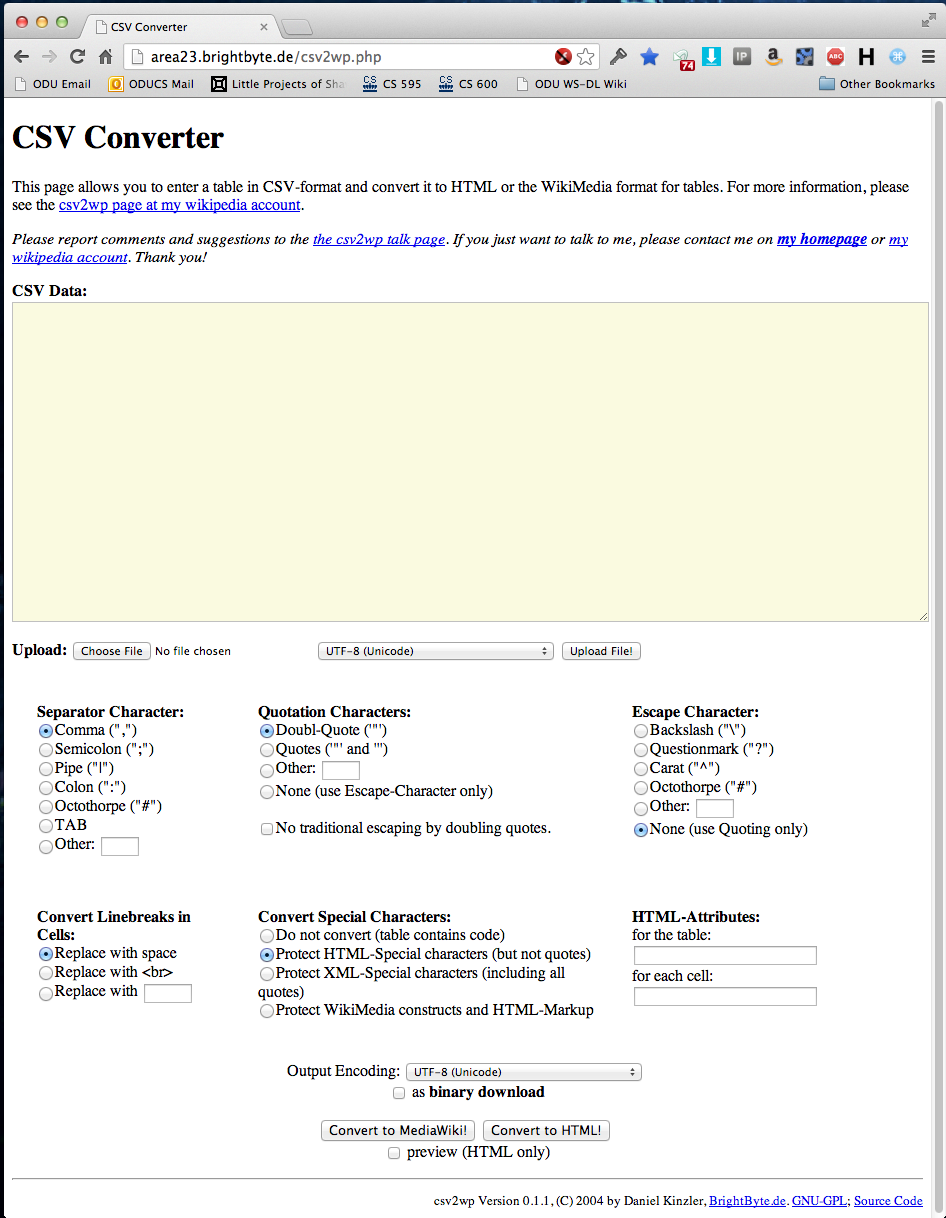
\includegraphics[scale=0.4]{work/q1screenie1.png}
\caption{The form for http://area23.brightbyte.de/csv2wp.php, rendered in Google Chrome}
\label{fig:q1screenie1}
\end{figure}

After reading the HTML, the form action is not shown, so the URI to POST to is also http://area23.brightbyte.de/csv2wp.php.

I posted the CSV data ``1,2'' to the form like so:
\begin{lstlisting}[frame=single]
curl -i --data 'csv=1,2&separator=,&quotes=&quot;&escape=\&break=SPACE&convert=html&output_encoding=UTF-8&to_wp=Convert+To+Mediawiki!'
   http://area23.brightbyte.de/csv2wp.php
\end{lstlisting}

and got back the following response from \verb+curl+:
\begin{lstlisting}[frame=single]
HTTP/1.1 200 OK
Date: Sat, 31 Aug 2013 23:20:02 GMT
Server: Apache/2.2.16 (Debian)
X-Powered-By: PHP/5.3.3-7+squeeze16
Content-Description: csv2wp-1377991202.UTF-8.txt
Content-Length: 23
Content-Type: text/plain; charset=UTF-8

{|
|1
|2
|----
|}
\end{lstlisting}

\newpage
Executing again, without -i, allows me to redirect the data to a file:
\begin{lstlisting}[frame=single]
curl --data 'csv=1,2&separator=,&quotes=&quot;&escape=\&break=SPACE&convert=html&output_encoding=UTF-8&to_wp=Convert+To+Mediawiki!'
   http://area23.brightbyte.de/csv2wp.php \
   > work/q1out.txt
\end{lstlisting}


which renders in the browser like shown in Figure \ref{fig:q1screenie2}.

\begin{figure}
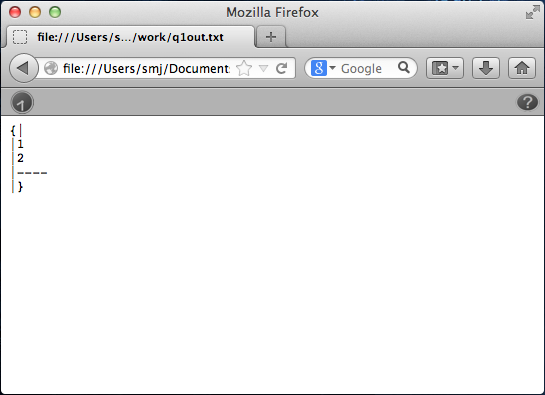
\includegraphics[scale=0.7]{work/q1screenie2.png}
\caption{The output of the curl command, rendered in Mozilla Firefox}
\label{fig:q1screenie2}
\end{figure}




\newpage
\section*{2}

\subsection*{Question}

Original:
\begin{verbatim}
Write a Python program that:
1. takes one argument, like "Old Dominion" or "Virginia Tech"
2. takes another argument specified in seconds (e.g., "60" for 
   one minute).
3. takes a URI as a third argument: 
   http://sports.yahoo.com/ncaa/football/scoreboard
   or
   http://sports.yahoo.com/ncaa/football/scoreboard?w=1&c=all&y=2012
   or
   http://sports.yahoo.com/ncaa/football/scoreboard?w=2&c=all&y=2012
   etc.
4. downloads the URI, finds the game corresponding to the team
   argument, prints out the current score (e.g., "Old Dominion 27, 
   East Carolina 17), sleeps for the specified seconds, and then
   repeats (until control-C is hit).
\end{verbatim}

\vfill
Updated Wed, September 4 10:31:37 EDT 2013:
\begingroup
\fontsize{8pt}{10pt}\selectfont
\begin{verbatim}
Write a Python program that:
1. takes one argument, like "Old Dominion" or "Virginia Tech"
2. takes another argument specified in seconds (e.g., "60" for 
   one minute).
3. takes a URI as a third argument, such as:
   http://scores.espn.go.com/ncf/scoreboard?confId=80&seasonYear=2013&seasonType=2&weekNumber=2
   or
   http://scores.espn.go.com/ncf/scoreboard?confId=80&seasonYear=2013&seasonType=2&weekNumber=1
   or
   http://scores.espn.go.com/ncf/scoreboard?confId=80&seasonYear=2012&seasonType=2&weekNumber=1
   etc.
4. downloads the URI, finds the game corresponding to the team
   argument, prints out the current score (e.g., "Old Dominion 38, 
   East Carolina 52), sleeps for the specified seconds, and then
   repeats (until control-C is hit).

   You can use any source for college football box scores that you'd like.
\end{verbatim}
\endgroup


\newpage
\subsection*{Answer}

\lstinputlisting[language=Python,frame=single,caption={Python program for acquiring NCAA Football scores from Yahoo sports},label=lst:q2code1,captionpos=b,numbers=left,showspaces=false,showstringspaces=false,basicstyle=\footnotesize]{work/gimmescore.py}

\newpage
The code is shown in Listing \ref{lst:q2code1} starting on page \pageref{lst:q2code1}:
\begin{itemize}
\item Takes an argument specifying the school (line 68)
\item Takes an argument specified in seconds (line 69)
\item Takes a URI as a third argument (line 70)
\item Downloads the URI (line 76), finds the game corresponding to the team argument (line 77), prints out the current score (line 79), sleeps for the specified seconds (line 82), and then repeats (line 75)
\end{itemize}

The core work is done in \emph{getScoresFromPage} (lines 30 to 63).  The trick to parsing the page is to realize that the actual data is inside HTML that is embedded in JavaScript defined inside one of the script tags.  The loop on line 37 searches all of the script tags for the given school.  Once the pertinent script tag is found, string replacement is done on line 42 to turn the JavaScript string into an actual HTML fragment, which is then fed into BeautifulSoup again, and a second search is performed on the actual entries.

The command is run like so:
\begin{lstlisting}[frame=single]
./gimmescore.py "Oregon" 10 http://sports.yahoo.com/ncaa/football/scoreboard
\end{lstlisting}

And produces output like the following:
\begin{lstlisting}[frame=single]
Nicholls 3, Oregon 66
Nicholls 3, Oregon 66
^CTraceback (most recent call last):
  File "./gimmescore.py", line 91, in <module>
  File "./gimmescore.py", line 87, in main
    
KeyboardInterrupt
\end{lstlisting}

After rerunning the script on September 9, 2013, it became evident that this implementation only worked for the September 2, 2013 and prior versions of the representation at http://sports.yahoo.com/ncaa/football/scoreboard.  Since that date, changes in the HTML to this page have rendered the script useless.

This is a common problem with ``screen scraping'' web pages, resulting in the re-writing of many tools.  Yahoo! has no obligation to continue to format their HTML as I expect, hence any such scripts can not be counted on to be permanent and should require frequent testing to remain valid.

Also, this script is very specific to this representation, meaning it will not work for a Fox Sports page or a CNN sports page.

\newpage
A corrected version of the script (gimmescore2.py) is shown in Listing \ref{lst:q2code2} on page \pageref{lst:q2code2}.  This script also includes improved error handling.

It is run and produces output like the following:
\begin{lstlisting}[frame=single]
bash $ --> ./gimmescore2.py "San Diego St." 10 "http://sports.yahoo.com/college-football/scoreboard/?week=2&conf="
San Diego St. 7, Ohio St. 42
San Diego St. 7, Ohio St. 42
^CTraceback (most recent call last):
  File "./gimmescore2.py", line 85, in <module>
  File "./gimmescore2.py", line 81, in main
    
KeyboardInterrupt

\end{lstlisting}

and the following (for a different week):
\begin{lstlisting}[frame=single]
bash $ --> ./gimmescore2.py "Virginia Tech" 10 "http://sports.yahoo.com/college-football/scoreboard/?week=1&conf="
Alabama 35, Virginia Tech 10
Alabama 35, Virginia Tech 10
Alabama 35, Virginia Tech 10
^CTraceback (most recent call last):
  File "./gimmescore2.py", line 98, in <module>
    main(sys.argv)
  File "./gimmescore2.py", line 92, in main
    time.sleep(refresh)
KeyboardInterrupt
\end{lstlisting}

If used against a school that isn't listed, it also gracefully recovers:
\begin{lstlisting}[frame=single]
bash $ --> ./gimmescore2.py "South Harmon Institute of Technology" 10 "http://sports.yahoo.com/college-football/scoreboard/?week=2&conf="
School "South Harmon Institute of Technology" not found in scores this week, maybe try again another day?
\end{lstlisting}

It also gracefully recovers from a game that hasn't started yet:
\begin{lstlisting}[frame=single]
bash $ --> ./gimmescore2.py "Vanderbilt" 10 "http://sports.yahoo.com/college-football/scoreboard/"
School "Vanderbilt" found, but game has not started yet
\end{lstlisting}

\newpage
And, of course, reports the scores while the game is running:

\begin{lstlisting}[frame=single]
bash $ --> ./gimmescore2.py "Troy" 60 "http://sports.yahoo.com/college-football/scoreboard/?conf=fbs_all"
Troy 14, Arkansas St. 20
Troy 14, Arkansas St. 20
Troy 14, Arkansas St. 20
Troy 20, Arkansas St. 20
Troy 20, Arkansas St. 20
Troy 21, Arkansas St. 20
^CTraceback (most recent call last):
  File "./gimmescore2.py", line 107, in <module>
    main(sys.argv)
  File "./gimmescore2.py", line 101, in main
    time.sleep(refresh)
KeyboardInterrupt
\end{lstlisting}

\newpage

\lstinputlisting[language=Python,frame=single,caption={Updated Python program for acquiring NCAA Football scores from Yahoo sports},label=lst:q2code2,captionpos=b,numbers=left,showspaces=false,showstringspaces=false,basicstyle=\footnotesize]{work/gimmescore2.py}


\newpage
\section*{3}

\subsection*{Question}

\begin{verbatim}
Consider the "bow-tie" graph in the Broder et al. paper (fig 9):
http://www9.org/w9cdrom/160/160.html

Now consider the following graph:

A --> B
B --> C
C --> D
C --> A
C --> G
E --> F
G --> C
G --> H
I --> H
I --> J
I --> K
J --> D 
L --> D
M --> A
M --> N
N --> D
    
For the above graph, give the values for:

IN: 
SCC: 
OUT: 
Tendrils: 
Tubes: 
Disconnected:
\end{verbatim}

\newpage
\subsection*{Answer}
Figure \ref{fig:q3graph} is a graph of the included points, generated using Graphviz.

\begin{figure}
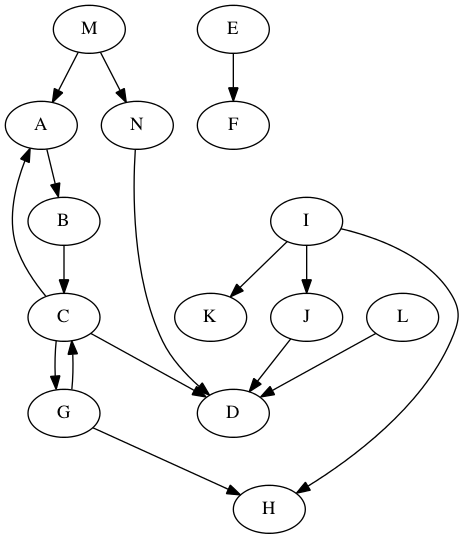
\includegraphics[scale=0.5]{work/q3.png}
\caption{Drawing of the example graph}
\label{fig:q3graph}
\end{figure}

The descriptions of each node is a matter of interpretation.  Explanations have been provided for each value assignment.

\textbf{IN:}  $M$

The IN components form the starting point for connection to the SCC\cite{broder2000}.  They all sit at the start of the graph.  In this graph, because of how the SCC and tubes are defined, the only IN component is $M$.

\textbf{SCC:}  $A, B, C, G$

The Strongly Connected Component consists of those heavily linked items connected to from the list of nodes listed as part of IN\cite{broder2000}.  It's an $A, B, C, G$ world.

\textbf{OUT:}  $D$

The OUT components exit the SCC, but do not link back to it\cite{broder2000}.  The only member of OUT is $D$, who forms a sink from members of the SCC and the tendrils.

\textbf{Tendrils:}  $I, J, K, L$

The \emph{Tendrils} are pages that cannot reach the SCC or are not reached from the SCC\cite{broder2000}.  The tendrils come from other graphs and only join the whole via $D$.

\textbf{Tubes:} $N$

Then there are \emph{tubes}, which pass from IN to OUT without going through SCC\cite{broder2000}.  $N$ is a tube linking from $M$ (from IN) to $D$ (from OUT).

\textbf{Disconnected:}  $E, F$

The Disconnected components link to no one in the graph, and stand alone.  They are not defined explicitly by Broder, et. al, but their meaning is implied within the paper.

\newpage
\bibliographystyle{acm}
\bibliography{references}


\end{document}